\documentclass{article}

\usepackage[version=3]{mhchem} % Package for chemical equation typesetting
\usepackage{siunitx} % Provides the \SI{}{} and \si{} command for typesetting SI units
\usepackage{graphicx} % Required for the inclusion of images
\usepackage{natbib} % Required to change bibliography style to APA
\usepackage{amsmath} % Required for some math elements 
\usepackage[labelformat=empty]{caption}
\usepackage[shortlabels]{enumitem}

\usepackage{listings}
\usepackage{graphicx}
\usepackage{xcolor}
\lstset { %
    language=C++,
    backgroundcolor=\color{black!5}, % set backgroundcolor
    basicstyle=\ttfamily,
    keywordstyle=\color{blue}\ttfamily,
    stringstyle=\color{red}\ttfamily,
    commentstyle=\color{gray}\ttfamily,
    morecomment=[l][\color{magenta}]{\#}
}


\setlength\parindent{0pt} % Removes all indentation from paragraphs

%\renewcommand{\labelenumi}{\alph{enumi}.} % Make numbering in the enumerate environment by letter rather than number (e.g. section 6)

%\usepackage{times} % Uncomment to use the Times New Roman font

%----------------------------------------------------------------------------------------
%	DOCUMENT INFORMATION
%----------------------------------------------------------------------------------------

\title{Algorytmy i Struktury Danych II \\ ZESTAW 02} % Title

\author{} % Author name

\date{} % Date for the report

\begin{document}

\maketitle % Insert the title, author and date

\begin{center}
\begin{tabular}{l r}
%Data labolatorium: & 29.03.2022 \\
Autor: & Marcin \textsc{Wolski}
\end{tabular}
\end{center}

\section*{(A) Funkcje hashujące}
Funkcje hashujące implementujące przyporządkowanie dla zbiorów:
\begin{enumerate}[a)] 
    \item liczb całkowitych $\mathbf{n, n+1, n+2, ...,m}$ gdzie n < m 
\begin{lstlisting}
int generateIndex (int number, int first) {
    return number - first;
}
\end{lstlisting}
    \item liczb całkowitych $\mathbf{n, n+2, n+4, ...,m}$ gdzie n < m
\begin{lstlisting}
int generateIndexEven (int number, int first) {
    return (number - first)/2;
}
\end{lstlisting}
    \item liter $\mathbf{a,b,c,...,z}$ bez polskich znaków ęóąśłżźć\\
\begin{lstlisting}
int generateIndexLetter (char letter) {
    return letter - 'a';
}
\end{lstlisting}
W C++ zmienna znakowa przechowuje wartość ASCII. Na przykład\\ wartość ASCII znaku "a" wynosi 97, "b" wynosi 98 itd. Wykorzystujemy ten fakt
do przypisywania miejsca w tablicy hashującej.
    \item dwuliterowych napisów, gdzie każda litera jest z zakresu $\mathbf{a - z}$ bez polskich znaków ęóąśłżźć
\begin{lstlisting}
int generateIndexLetterPair 
                    (char letter1, char letter2) {
    return (letter1 - 'a')*26 + (letter2 - 'a');
}
\end{lstlisting}
\end{enumerate}

\section*{(B) Typ danych setHashed}
 Typ danych setHashed, wykorzystujący haszowanie otwarte, reprezentuje\\ matematyczny zbiór oraz operacje które dla dwóch zbiorów realizują: 
\begin{itemize} 
    \item sumę zbiorów
    \item część wspólną zbiorów
    \item różnicę zbiorów
    \item sprawdzanie identyczności zbiorów
\end{itemize}
oraz dla elementu zbioru realizują: 
\begin{itemize}
    \item wstawanie elementu do zbioru
    \item usuwanie elementu ze zbioru
    \item sprawdzanie czy element należy do zbioru
\end{itemize}

\subsection*{Badanie złożoności operacji}
 Czas wykonania operacji zmierzony został dla zbiorów o rozmiarach [1, 500]. Dla każdej wielkości obliczona została średnia z 1000 powtórzeń działania. Wygenerowane zostały pliki z danymi które zwizualizowane zostały za pomocą programu gnuplot.

\subsection*{Wykresy}
Pionowa oś - czas w nanosekundach\\
Pozioma oś - rozmiar problemu\\
\begin{center}
    \textit{Wstawianie elementu, mala ilosc binów (25)\\}
    \includegraphics[width=0.5\textwidth]{insert_bins25}\\
    \textit{Wstawianie elementu, duza ilosc binów (500)\\}
    \includegraphics[width=0.5\textwidth]{insert_bins500}\\
    \textit{Różnica dwóch zbiorów\\}
    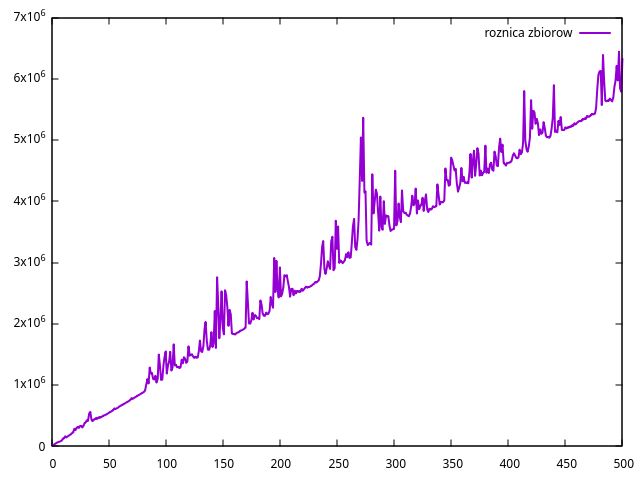
\includegraphics[width=0.5\textwidth]{difference}\\
    \textit{Przecięcie dwóch zbiorów\\}
    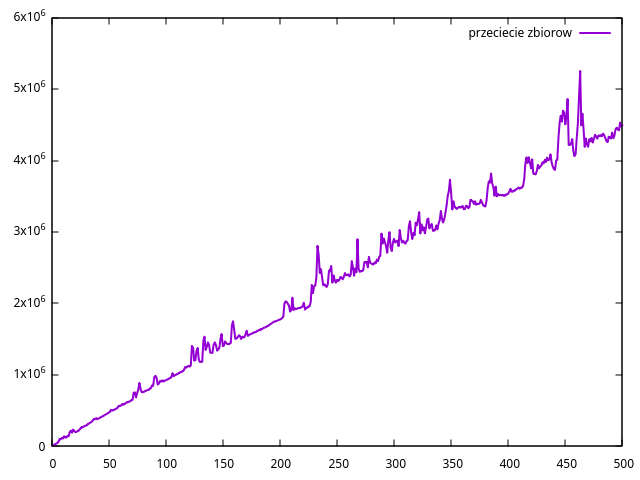
\includegraphics[width=0.5\textwidth]{intersection}\\
    \textit{Suma dwóch zbiorów\\}
    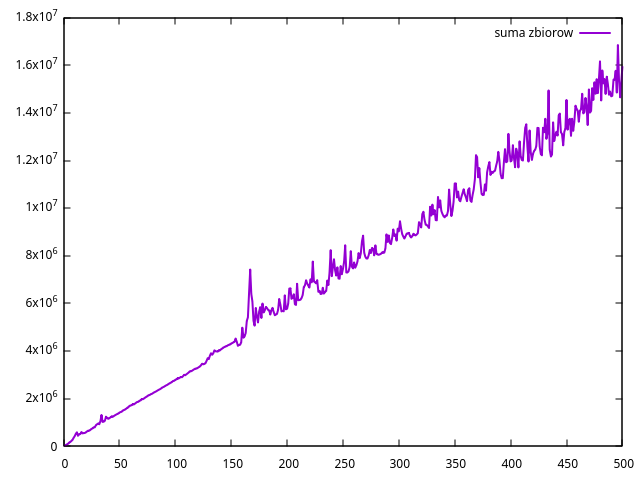
\includegraphics[width=0.5\textwidth]{unify}\\
\end{center}

\section*{(C) Porównanie implementacji}
Porównanie implementacji zbioru z zadań A i B z zestawu 1 i zbioru haszującego z zadania B z obecnego zestawu.\\\\
Wartości zbioru z zadania A z pierwszego zestawu nie są związane z konkretnymi kluczami. Są poindeksowane sekwencyjnie w tablicy. Randomowy dostęp do elementu wynosi O(1), a do konkretnego elementu (musi przeszukać tablice po kolei) wynosi O(n).\\

W zbiorze z zadanie A z pierwszego zestawu wartości również nie są powiązane z kluczami. Dostęp jest sekwencyjny (przeszukiwanie od pierwszego węzła).\\

Zbiór hashujący, dzięki cechom słownika(tablicy asocjacyjnej), pozwala na szybkie wstawianie, wyszukiwanie i usuwanie. Przy każdej operacji odwołujemy się do indeksu zwróconego przez funkcję haszującą. Zbiór haszujący zaimplementowany został na bazie tablicy list wiązanych.\\ Przy przeszukiwaniu, w najgorszym przypadku wszystkie klucze wskazują na jeden slot tablicy i struktura staje się porównywalna do listy wiązanej. To oznacza że operacje mają złożoność O(n).\\ 
Zakładając jednak, że klucze są rozmieszczone równomiernie, można oczekiwać złożoności wynoszącej O(1).

\subsection*{Której implementacji najlepiej użyć?}
W przypadku gdy w naszym zbiorze dane posiadają charakterystyczny klucz który je definiuje, lepiej wykorzystać zbiór haszujący. Dostęp do konkretnego elementu będzie wynosił O(1) przy równomiernie rozłożonych wartościach.\\ 

Jeśli zależy nam bardziej na dostępie do randomowego elementu w zbiorze, lepiej wykorzystać setSimple, złożoność O(1).\\

Jeśli randomowy dostęp nie jest istotny i wartości nie są powiązanie z kluczami, a zależy nam na dynamicznym zbiorze (łatwe usuwanie, dodawanie), możemy wykorzystać setLinked.
\cite{}
\end{document}